%-----------------------------------------------------
% Chapter: Methodology
%-----------------------------------------------------
\chapter{Methodology}
This chapter details the methodology used to collect, analyse and process the dataset used to derive the CoVeR word embeddings.
\label{chap:data_methodology}
\section{Collecting Data}
As previously mentioned, there exists no central repository from which song lyrics can be obtained. Though lyric hosting websites such as Genius(FOOTNOTE) exist, selective collection of song lyrics is only achievable through the process of web scraping. Web scraping is the process of exhaustively downloading web pages, from either a predefined list of URLs or through link extraction. Large scale scraping is usually achieved through parallelised methods due to restrictions such as Robots.txt and download latency. Taking into account the project objectives and goals, web scraping was avoided.

\noindent
\newline
In view of this, a publicly available dataset containing over 250,000 lyrics was used. The dataset comprised of two .csv files: artists and lyrics. The artists .csv file mapped individual artists to their respective genres/sub genres, whilst the lyrics .csv file contained data on individual songs, mapping lyrics to artists. 
\section{Data Analysis and Restructuring}
The CoVeR algorithm requires sub corpora to be labelled in order to jointly learn word embeddings and the relevant transformation matrices. With regards to this project a mapping between lyrics and genre was required. To fulfil this requirement Pandas, a Python data manipulation/analysis library was used  perform a SQL like join on both sets of data, specifically on the artist name.

\noindent
\newline
100,000 song lyrics were decided on to be used as training data. A trivial approach to split the data on the genre covariate would involve an equal split for equal representation, however, this method has the assumption that for each particular genre, word usage is the same on average. 

\begin{figure}[h]
	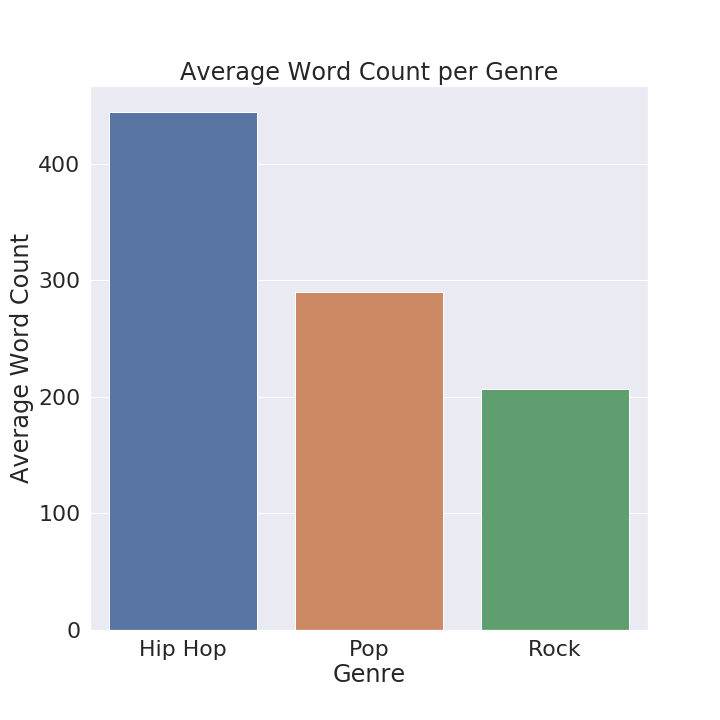
\includegraphics[width=8cm, height=8cm]{./figures/fig6}
	\centering
	\caption{Average word count per lyric per genre in the dataset}
	\label{fig:fig6}
\end{figure}

\noindent
\newline
Examining the dataset proved this not to be the case, with Hip-Hop songs containing 444 words on average compared to the 207 found in Rock songs and 289 found in Pop songs. To reflect these statistics in the training data, a training split of 48:30:22 for Rock, Pop and Hip-Hop was used.
\section{Data Pre-processing}
Essential to any machine learning task is the pre-processing of input data in such a way that important features are accessible during training. In natural language processing, this can include techniques such as tokenisation, string cleaning, stemming and lemmatisation. 

\noindent
\newline
Following the lyric data reconstruction, each lyric in the corpus was cleansed and tokenised. The following string cleaning techniques were applied to each lyric in the dataset.

\begin{enumerate}
	\item All letters were lowercased.
	\item All characters, except for letters, were substituted with a space " ".
	\item All text between brackets were removed. (This was to ensure text like \textbf{[Verse 1]} was not included during training).
	\item All trailing white space was removed.
\end{enumerate}

\noindent
\newline
Tokenisation is the process of separating textual inputs into meaningful chunks called \textit{tokens}. Naturally to create word embeddings, text is tokenised at the word level and each token has a one-one mapping with a unique numerical key, which is used to transform each lyric in the corpus into a list of numerical keys. For training, only tokens which appeared a minimum number of times were kept.
 
\noindent
\newline
Typically found within text corpora are high frequency stop words such as 'the', 'a', and 'in' which provide less information than rarely occurring words(REF-DISTRIBUTED REP OF WORDS). For example... This concept can also be applied to word embeddings; where the word embeddings of frequent words does not change significantly after training on several examples. Similar to (REF), subsampling was used at the covariate level using the following adapted formula from the original word2vec implementation.

\begin{equation}
P(w_{ik}) = \sqrt{\dfrac{z(w_{ik})}{t}} + 1 \cdot \dfrac{t}{z(w_{ik})}
\end{equation}

\noindent
\newline
where \(z(w_{ik})\) is the percentage of word \(w_{ik}\) in covariate \(k\) and \(t\) is a chosen threshold.

\section{Hyperparameters}
\subsection{CoVeR}
\subsubsection{Embedding Size}
\subsubsection{Optimiser}
\subsubsection{Window Size}
\subsubsection{Asymmetric vs Symmetric Windows}
\subsection{Language Model}
\subsection{Text Classifier}

